\documentclass[12pt]{article}
\usepackage[margin=0.8in]{geometry}
\usepackage{amsmath}
\usepackage{hyperref}
\usepackage{graphicx}
\usepackage{float}
\usepackage{caption}
\usepackage{subcaption}

\title{Numerical analysis: Assignment 5}
\author{Niccolo Zuppichini}
\begin{document}

\maketitle
\section*{Exercise 1}

We want to interpolate n + 1 points P0 ... Pn given n + 7 knots points $t_i$. In order to do this we need do compute the control points D. The control points are calculated by solving the system $MD = P$ where M is a tridiagonal matrix containing the B-spline basis. \\
In order to compute the basis the recursive definition has been employed. 

\begin{equation}
	N_i^0(t) =
	\begin{cases}
		1 \quad \textrm{for} t \in [t_i, t_{i+1}) \\
		0 \quad \textrm{else}
	\end{cases}
	\quad \textrm{for} i = 0, ..., 2n + m
\end{equation}

\begin{equation}
	N_i^j = \frac{t - t_i}{t_{i+j} - t_i} N^{j-1}_i + \frac{t_{i+j+1} - t}{t_{i+j+1} - t_i} N^{j-i}_{i+1}
\end{equation}


Then we populate the tridiagonal matrix M using those basis functions. We have a tridiagonal matrix because each basis N has local support. \\

I was not able  to compute the natural end conditions, therefore the first and last rows of the matrix are missing and so the matrix is not square. This means that I can't use the Thomas algorithm to solve it efficiently. However, I've implemented the tridiagonal solver (code in \textit{code.py}) anyway, but since my matrix is missing 2 rows I haven't used it (after employing the natural conditions it can be used). I've solved the system using the least square method included in the scipy library, instead. \\
After evaluating the control points, I've De Boor’s algorithm to evaluate the b-spline. \\

\begin{figure}[H]
\centering
\begin{subfigure}{.5\textwidth}
  \centering
	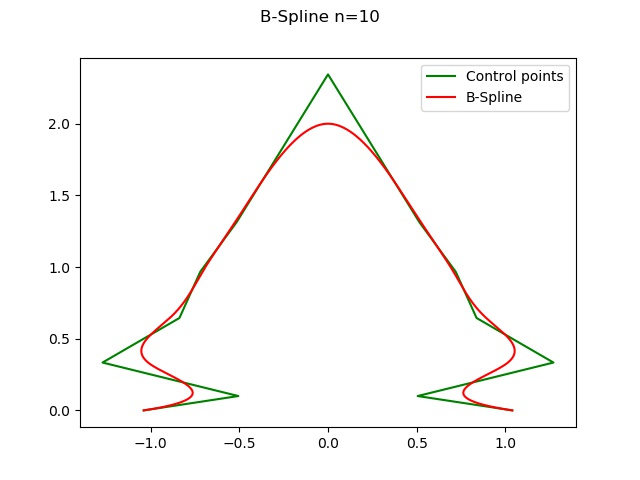
\includegraphics[width=0.7\columnwidth]{result10.jpg}
	\caption{n=10}
%	\label{fig:result}
\end{subfigure}%
\begin{subfigure}{.5\textwidth}
 \centering
	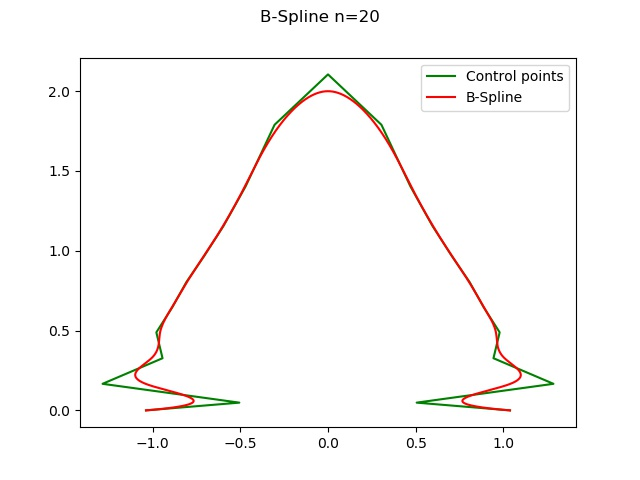
\includegraphics[width=0.7\columnwidth]{result20.jpg}
	\caption{n=20}
%	\label{fig:result}
\end{subfigure}
\begin{subfigure}{.5\textwidth}
 \centering
	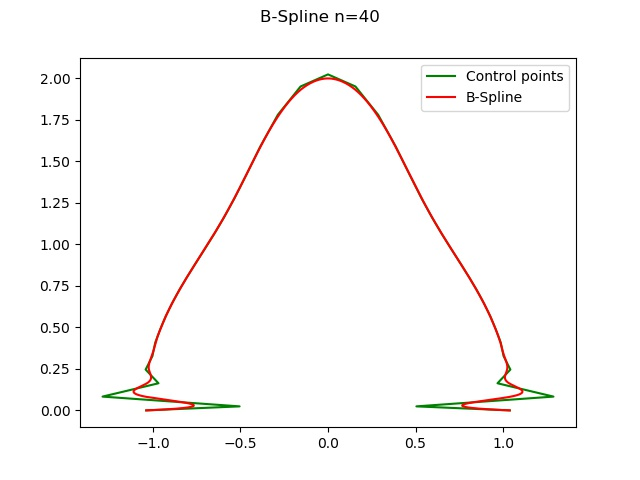
\includegraphics[width=0.7\columnwidth]{result40.jpg}
	\caption{n=40}
%	\label{fig:result}
\end{subfigure}
\caption{Result from my python implementation. The red curve is my b-spline and the green polygon is the control polygon.}
\label{fig:result}

\end{figure}


Figure \ref{fig:result} shows that the function interpolates the points correctly. Moreover, it is more stable than the interpolation polynomial computed in exercise 4 (which had stability problems at the boundaries). \\

\section*{Exercise 2}
Unfortunately I ran out of time.


\end{document}